\chapter{Dasar Teori}
\label{chap:teori}
Bab ini berisi dasar teori dari pembangunan Aplikasi Pencarian Rute Kendaraan Umum untuk Windows Phone. Beberapa teori yang dibahas dalam bab ini  adalah Kiri API, Web Service, Menampilkan Peta, Penggunaan \textit{Global Positioning System} di Windows Phone, dan antarmuka perangkat lunak yang dibuat. 

% Windows Phone
\section{Windows Phone}
\label{sec:Windows Phone}
\hspace{0.5cm} Sub bab ini akan membahas pemrograman di Windows Phone. Pembahasan akan dimulai dengan apa itu Windows Phone dan fitur di Windows Phone yang akan digunakan dalam pembangunan perangkat lunak Pencarian Rute Kendaraan di Windows Phone. 

Windows Phone merupakan sistem operasi untuk perangkat bergerak yang dikembangkan Microsoft.\footnotemark[1] Untuk mengembangkan aplikasi Windows Phone dibutuhkan Windows Desktop 8 sebagai media pengembangan. Bahasa pemrograman yang digunakan untuk membuat perangkat lunak di Windows Phone yaitu C\# dan Visual Basic.  
%kutipan mengenai windows phone
\footnotetext[1]{\url{en.wikipedia.org/wiki/Windows_Phone}}

% Lingkungan Kerja
\subsection{Lingkungan Kerja}
\label{subsec:Lingkungan Kerja}
\hspace{0.5cm} Microsoft .NET framework merupakan sebuah perangkat lunak yang dibangun untuk membantu dalam pembangunan aplikasi di Windows, Windows Phone, Windows Server, and Microsoft Azure\footnotemark[2]. Ini terdiri dari runtime bahasa umum dan perpustakaan kelas NET Framework, yang meliputi kelas, interface, dan jenis nilai yang mendukung berbagai teknologi. NET Framework menyediakan lingkungan yang mudah dikelola, pengembangan disederhanakan dan penyebaran, dan integrasi dengan berbagai bahasa pemrograman, termasuk Visual Basic dan Visual C\#.
\hspace{0.5cm} Seperti yang telah disebutkan ada dua bahasa pemrograman dalam .NET Framework yang dipakai dalam pembangunan aplikasi di Windows Phone 8 yaitu Visual Basic dan Visual C\#. Untuk masalah kehandalan keduanya menawarkan kehandalan yang baik. Kelebihan dari Visual Basic adalah bahasa pemrograman berorientasi objek yang kuat dan memiliki banyak pengenbangan fitur di inheritance, polymorphism, interfaces, and overloading\footnotemark[3].Kelebihan dari C\# yang merupakan pengembangan dari C/C++ adalah sederhana, modern, aman dan berorientasi objek\footnotemark[4]. Satu hal yang dirasakan penulis adalah kenyamanan ketika memilih bahasa .NET tersebut. Akan lebih mudah bagi developer yang menggunakan Visual Basic 6.0  untuk menggunakan Visual Basic .NET. Tetapi bagi  deveoper yang menggunakan C++ atau java sebelumnya akan lebih mudah menggunakan C\#.
%kutipan mengenai .NET
\footnotetext[2]{\url{http://msdn.microsoft.com/en-us/library/vstudio/w0x726c2\%28v=vs.110\%29}}
\footnotetext[3]{\url{http://msdn.microsoft.com/en-us/library/aa903378\%28v=vs.71\%29.aspx}}
\footnotetext[4]{\url{http://msdn.microsoft.com/en-us/library/aa287558\%28v=vs.71\%29.aspx}}

% SUB Mengenai XAML
\subsection{XAML}
\label{subsec:XAML}
\hspace{0.5cm} Extensible Application Markup Language (XAML) merupakan bahasa deklaratif yang dipakai untuk membuat antarmuka aplikasi. XAML merupakan bahasa yang digunakan untuk membuat antarmuka di Windows Phone 8. Pada dasarnya penggunaan XAML sama dengan HTML pada pembuatan antarmuka web. XAML dapat menginisialisasi objek dan mengatur properti untuk menunjukan hubungan antar objek.
\hspace{0.5cm} Untuk aturan penulisan sintak XAML didasarkan pada XML. Setiap XAML Windows Runtime menggunakan konvensi XAML language dan ditulis pada \textit{namespace} yang ditandai dengan prefix x sebagai elemen paling atas. Setelah itu di baris ke dua dimulai dengan xmlns diikuti titik dua, lalu nama dari \textit{namespace}, diikuti tanda sama dengan dan \textit{path} perepresentasian \textit{namespace}.
Prefix x pada XAML mengandung beberapa struktur program yang sering kita gunakan yaitu :
\begin{itemize}
	\item x:Key : sebuah nama unik untuk menunjuk referensi ke suatu resource atau berkas lain. Nilai ini dapat dipanggil kembali untuk menggunakan resource tersebut.
	\item x:Class : menunjukkan nama kelas.
	\item x:Name : menunjukkan nama sebuah obyek dan untuk membedakan antar obyek yang satu dengan obyek yang lain.
	\item x:Uid : mengidentifikasi elemen objek dalam XAML. Objek elemen merupakan objek yang dapat melakukan kontrol terhadap kelas atau elemen lain yang ditampilkan di desain anarmuka.
\end{itemize}	

% SUB Mengenai Kontrol terhadap Ponsel
\subsection{Kontrol terhadap Ponsel}
\label{subsec:Kontrol terhadap Ponsel}
\hspace{0.5cm} Kontrol terhadap ponsel yang dimaksudkan disini adalah pengaturan tata letak terhadap antarmuka di Windows Phone. Windows Phone 8 menyediakan banyak set kontrol yaitu tata letak, tombol, kontrol masukan untuk mendapatkan informasi sampai ke menu. 

% SUB SUB Navigasi
\subsubsection{Navigasi}
\label{subsubsec:Navigasi}
\hspace{0.5cm} Aplikasi yang dibuat di Windows Phone didasarkan pada model halaman. Maksud dari model halaman adalah pengguna berpindah dari satu halaman ke halaman lain dengan konten yang berbeda-beda dengan frame sebagai pengontrolnya. Setiap antarmuka aplikasi dibungkus dengan frame. Frame inilah yang melakukan kontrol terhadap aplikasi dan memungkinkan berpindah dari satu halaman ke halaman lain. Sedangkan halaman merupakan pembungkus dari elemen di dalamnya saja. Untuk lebih jelas mengenai frame, halaman dan area konten dapat dilihat pada gambar di bawah ini.

\begin{figure}[h]
	\centering
		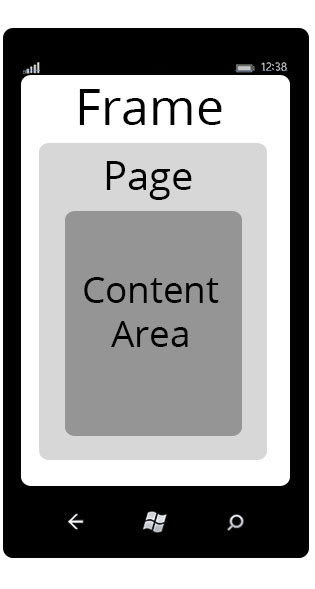
\includegraphics[scale=0.5]{Gambar/nav_hierarchy.jpg}
	\caption{Hirarki Navigasi}
	\label{fig:nav_hierarchy}
\end{figure}


% SUB SUB Mengenai Tata Letak
\subsubsection{Kontrol Tata Letak}
\label{subsubsec:Kontrol Tata Letak}
\hspace{0.5cm} Kontrol Tata Letak merupakan penampung pada antarmuka Windows Phone untuk objek di antarmuka dan kontrol yang lain (tombol radio, textbox, dan lai-lain). Kontrol tata letak digunakan untuk meletakan objek-objek di layar. Ketika pertama membuat aplikasi Windows Phone maka tata letak dasar sebagai penampung akan langsung dibuat berikut panel judul dan panel konten. Selanjutnya untuk penambahan kontrol tata letak yang lain dapat ditambahkan di panel konten.


\hspace{0.5cm} Ada 3 macam panel yang dipakai untuk menangani Tata Letak yaitu Grid, StackPane, dan Canvas. Perlu diperhatikan bahwa setiap halaman hanya memiliki satu macam panel. Berikut 3 macam panel di Windows Phone:

\begin{itemize}
	\item StackPanel merupakan panel yang memposisikan element menjadi 1 baris dan beberapa elemen di setiap halaman diposisikan horizontal atau vertical saja.
	\item Grid merupakan panel yang mendukung tata letak yang rumit. Panel ini memposisikan elemen di baris dan kolom mana saja di setiap halaman.
	\item Canvas memposiskan elemen sebagai absolut kordinat. Jadi setiap elemen di dalam Canvas dapat diposisikan spesifik sesuai kordinat x dan y.
\end{itemize}
	
% SUB SUB Mengenai Kontrol Masukan
\subsubsection{Kontrol Terhadap Teks}
\label{subsubsec:Kontrol Terhadap Teks}
\hspace{0.5cm} Kontrol Terhadap Teks  secara menampilkan konten String. Ada berbagai macam Kontrol Terhadap Teks di Windows Phone yaitu TextBlock, TextBox dan PasswordBox. Ketiga macam kontrol tersebut dibedakan menurut tujuannya. Berikut gambar dan keterangan masing-masing:
\begin{figure}[h]
	\centering
		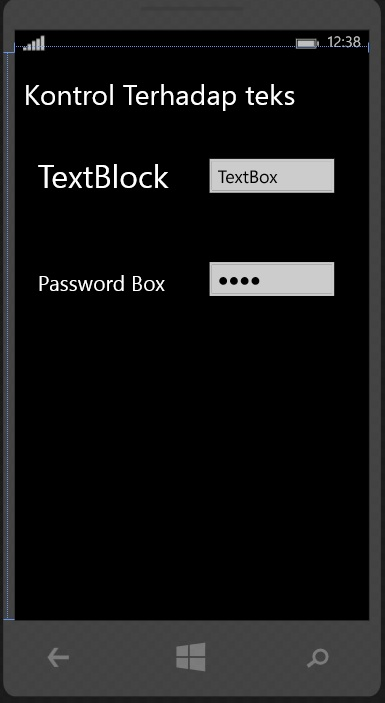
\includegraphics[scale=0.5]{Gambar/Tombol/kontrol_teks}
	\caption{TextBlock, TextBox dan PasswordBox}
	\label{fig:kontrol_teks}
\end{figure}

\begin{itemize}
	\item TextBlock merupakan tempat menaruh potongan teks yang hanya bisa dilihat.
	\item TextBox biasanya digunakan untuk teks masukan yang pendek. Tapi bisa juga dipakai untuk masukan yang banyak dan beberapa baris.
	\item PasswordBox biasanya digunakan untuk masukan yang bersifat rahasia. Karakter yang dimasukan langsung disamarkan menjadi bentuk titik.
\end{itemize}

% SUB SUB Mengenai Kontrol Masukan
\subsubsection{Tombol dan Kontrol Pilihan}
\label{subsubsec:Tombol dan Kontrol Pilihan}
\hspace{0.5cm} Tombol memungkinkan pengguna untuk bernavigasi. Sedangkan kontrol pilihan memudahkan dalam memilih. Berikut gambar dan keterangan masing-masing:
 
\begin{figure}[h]
	\centering
		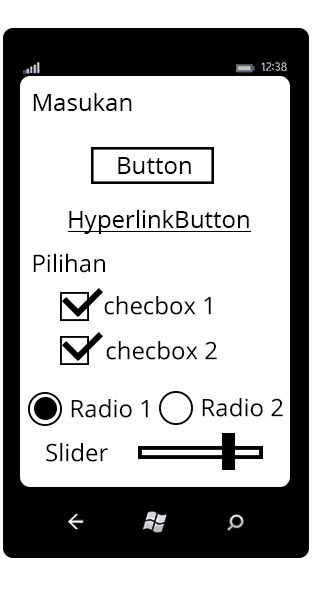
\includegraphics[scale=0.5]{Gambar/Tombol/tombol_dan_pilihan}
	\caption{TextBlock, TextBox dan PasswordBox}
	\label{fig:kontrol_tombol}
\end{figure}

\begin{itemize}
	\item Button merupakan kontrol yang dipakai pengguna untuk mengaktifkan \textit{event} klik.
	\item HyperlinkButton merupakan kontrol yang menampilkan hyperlink. Jika di tekan maka akan menunjuk ke halaman yang dituju.	
	\item CheckBox merupakan kontrol yang memungkinkan pengguna memilih beberapa item.
	\item RadioButton merupakan kontrol yang memungkinkan pengguna memilih satu pilihan dari beberapa pilihan.
	\item Slider merupakan kontrol yang memungkinkan user memilih nilai kisaran dari jalur yang sudah disediakan.
\end{itemize}

% SUB SUB Kontrol Daftar
\subsubsection{Kontrol Daftar}
\label{subsubsec:Kontrol Daftar}
\hspace{0.5cm} Kontrol yang dipakai untuk menampilkan daftar dari beberapa item. Berikut keterangan masing-masing:

\begin{itemize}
	\item ListBox akan menampilkan daftar item. Daftar ini dapat dipilih dengan cara di klik.
	\item LongListSelector dipakai untuk mengelompokan, menampilkan, dan melakukan penggulungan terhadap daftar yang panjang.
\end{itemize}

% SUB SUB Gambar, Peta, dan Media
\subsubsection{Gambar, Peta, dan Media}
\label{subsubsec:Gambar, Peta, dan Media}
\hspace{0.5cm} Menampilkan gambar, map, dan konten media penting sebagai bagian dari antarmuka. Berikut keterangan masing-masing:

\begin{itemize}
	\item Image dipakai untuk menampilkan gambar. Aplikasi di Windows Phone mendukung format jpeg dan png. 
	\item Map dipakai menampilkan peta.
	\item MediaElement dipakai untuk memainkan audio dan video.
\end{itemize}

% SUB Mengenai Lifecycle
\subsection{Lifecycle Windows Phone}
\label{subsec:Lifecycle Windows Phone}

\begin{itemize}
	\item Running : Aplikasi sedang berada di bagian depan. Hanya satu aplikasi yang diijinkan berada di depan pada satu waktu.
	\item Dormant : Aplikasi tidak berada di bagian depan, tetapi sistem operasi tidak membutuhkan sumber daya(dalam hal ini memori). Pada tahap ini objek aplikasi masih berada di memori, jadi pada tahap Dormant aplikasi dapat secara otomatis diaktifkan kembali. Tetapi jika sistem operasi  membutuhkan sumbe daya maka aplikasi akan menjadi \textit{tombstoned} dan dihancurkan. 
	\item Tombstoned : Aplikasi akan dihancurkan dan objek aplikasi akan dihapus dari memori. Ketika aplikasi diaktivasi pengguna akan ditempatkan kembali di halaman yang ditinggalkan sebelumnya, tetapi objek harus di kembalikan dari keadaan sebelumnya.
\end{itemize}

% SUB SUB Penyimpanan dan Pengembalian Keadaan Aplikasi
\subsubsection{Penyimpanan dan Pengembalian Keadaan Aplikasi}
\label{subsubsec:Penyimpanan dan Pengembalian Keadaan Aplikasi}

\begin{lstlisting} [caption= App.xaml]
	<Application.ApplicationLifetimeObjects>
		<!--Required object that handles lifetime events for the application-->
		<shell:PhoneApplicationService
			Launching="Application_Launching" Closing="Application_Closing"
			Activated="Application_Activated" Deactivated="Application_Deactivated"/>
	</Application.ApplicationLifetimeObjects>
\end{lstlisting}

\begin{lstlisting} [caption= Appp.xaml.cs]
	// Code to execute when the application is launching (eg, from Start)
	// This code will not execute when the application is reactivated
	private void Application_Launching(object sender, LaunchingEventArgs e)
	{
	}
	// Code to execute when the application is activated (brought to foreground)
	// This code will not execute when the application is first launched
	private void Application_Activated(object sender, ActivatedEventArgs e)
	{
	}
	// Code to execute when the application is deactivated (sent to background)
	// This code will not execute when the application is closing
	private void Application_Deactivated(object sender, DeactivatedEventArgs e)
	{
	}
	// Code to execute when the application is closing (eg, user hit Back)
	// This code will not execute when the application is deactivated
	private void Application_Closing(object sender, ClosingEventArgs e)
	{
	}
\end{lstlisting}

\begin{lstlisting} [caption= Penanganan terhadap pengaktifan dan penonaktifan kejadian]
	public class MyObject
	{
	public DateTime LastUpdate { get; set; }
	}
	//...
	public MyObject MyObject { get; set; }
	
	private void Application_Activated(object sender, ActivatedEventArgs e)
	{
		DateTime lastUpdate =
		(DateTime)PhoneApplicationService.Current.State["LastUpdate"];
		Debug.WriteLine("Application_Activated: LastUpdate=" + lastUpdate.ToLongTimeString());
	}
	private void Application_Deactivated(object sender, DeactivatedEventArgs e)
	{
		Debug.WriteLine("Application_Deactivated: Saving LastUpdate to application state");
		PhoneApplicationService.Current.State["LastUpdate"] = DateTime.Now;
	}
\end{lstlisting}

% SUB Peta di Windows Phone
\subsection{Peta di Windows Phone}
\label{subsec:Peta di Windows Phone}
\hspace{0.5cm} Peta untuk Windows Phone adalah Here Maps. Here Maps yang akan menampilkan lokasi dan melakukan penelusuran. Pada Sub Bab ini akan dibahas mengenai penambahan peta pada aplikasi, mendapatkan lokasi, petunjuk arah dan Pushpins.

% SUB SUB Mengenai Penambahan Maps Ke Aplikasi
\subsubsection{Penambahan Maps Ke Aplikasi}
\label{subsubsec:Penambahan Maps Ke Aplikasi}
\hspace{0.5cm} Ada dua cara untuk menambahkan peta ke aplikasi yang pertama dengan menjalankan MapTask dan yang kedua dengan ppenambahan ID\_CAP\_MAP ke \textbackslash properties\textbackslash WMAppManifest.xml. Contoh dibawah adalah dengan MapTask yang memenggil metode Show() untuk memunculkan peta.

\begin{lstlisting} [caption= code pemanggilan maps]
	private void MapClick(object sender, EventArgs e)
	{
		var task = new MapsTask();
		var goldenGateBridge = new GeoCoordinate(37.8085880, -122.4770175);
		task.Center = goldenGateBridge;
		task.ZoomLevel = 9;
		task.SearchTerm = "Golden Gate Bridge";
		task.Show();
	}
\end{lstlisting}

\begin{lstlisting} [caption= penambahan Map Element menggunakan Map Control]
	<Grid x:Name="LayoutRoot" Background="Transparent">
		<Controls:Map x:Name="WorldMap" />
	</Grid>
\end{lstlisting}

% SUB SUB Mengenai Posisi Pada Peta
\subsubsection{Posisi Pada Peta}
\label{subsubsec:Posisi Pada Peta}
\hspace{0.5cm} Ketika memulai membuka peta maka akan menampilkan seluruh dunia dan pengguna harus melakukan \textit{pinch-and-zoom} untuk melihat titk tertentu. Agar dapat memudahkan pengguna dalam memilih titik tertentu secara otomatis maka dapat menggunakan metode SetView\(\). Pada Listing dibawah dapat dilihat bahwa SetView\(\) memiliki 2 parameter. Parameter pertama menyatakan tempat dengan GeoCordinate yang mendefinisikan pusat pandangan. Selanjutnya parameter ke 2 merupakan zoomLevel ( 1 = zoomed out, 20 = zoomed in). 

\begin{lstlisting} [caption= Posisi Pada Peta]
	GeoCoordinate GoldenGateBridge = new GeoCoordinate(37.8085880, -122.4770175);
	SanFranciscoMap.SetView(GoldenGateBridge, 15);
\end{lstlisting}

% SUB SUB Penambahan Pushpins ke Peta
\subsubsection{Penambahan Pushpins ke Peta}
\label{subsubsec:Penambahan Pushpins ke Peta}

\hspace{0.5cm} Peta tidak mendukung langsung cara untuk mengikat data ke MapLayer dan MapOverlay. Untungnya di Windows Phone memiliki Windows Phone 8 Toolkit yang memiliki set objek yang dapat digunakan sebagai jembatan mengikat data ke MapLayer dan MapOverlay.

\begin{lstlisting} [caption= Berikut contoh Tookkit Pushpin dengan elemen-element yang di tulisa manual]
	<Controls:Map>
		<Toolkit:MapExtensions.Children>
			<Toolkit:Pushpin Content="London" GeoCoordinate="51.499493,-0.124753" />
		</Toolkit:MapExtensions.Children>
	</Controls:Map>
\end{lstlisting}

\hspace{0.5cm} Gambar dibawah merupakan keluaran di peta. Label "London" merupkan bawaan Windows Phone 8 pushpin.

\begin{figure}[!h]
	\centering
		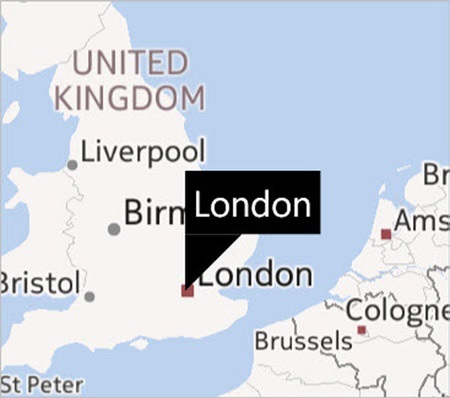
\includegraphics[scale=0.5]{Gambar/toolkit_pushpin.jpg}
	\caption{Keluaran Toolkit Pushpin pada Peta}
	\label{fig:toolkit_pushpin}
\end{figure}

\hspace{0.5cm} Selain menetapkan Pushpin secara langsung  di MapExtensions, dapat pula diletakan MapItemsControl. Pushpin akan berpindah ke ItemTemplate dan ItemSource akan ditugaskan ViewModel.

\begin{lstlisting} [caption= Berikut contoh Tookkit Pushpin dengan elemen-element yang di tulisa manual]
	<Controls:Map x:Name="WorldMap" >
		<Toolkit:MapExtensions.Children>
			<Toolkit:MapItemsControl ItemTemplate="{StaticResource MapItemTemplate}" ItemsSource="{Binding Source={StaticResource LocationViewModel}, Path=Locations}" />
		</Toolkit:MapExtensions.Children>
	</Controls:Map>
\end{lstlisting}

\begin{lstlisting} [caption= View Model]
	public class Location
	{
		public string Title { get; set; }
		[TypeConverter(typeof(GeoCoordinateConverter))]
		public GeoCoordinate GeoCoordinate { get; set; }
	}
	
	public class LocationViewModel
	{
		public ObservableCollection<Location> Locations { get; set; }
		public LocationViewModel()
		{
			Locations = new ObservableCollection<Location>();
		}
	}
\end{lstlisting}

\begin{lstlisting} [caption= Deklarasi View Model]
	<phone:PhoneApplicationPage.Resources>
		<vm:LocationViewModel x:Key="LocationViewModel" >
			<vm:LocationViewModel.Locations>
				<vm:Location Title="London" GeoCoordinate="51.499493,-0.124753" />
				<vm:Location Title="Paris" GeoCoordinate="48.858222,2.2945" />
				<vm:Location Title="Rome" GeoCoordinate="41.890268,12.492315" />
			</vm:LocationViewModel.Locations>
		</vm:LocationViewModel>
		<DataTemplate x:Name="MapItemTemplate">
			<Toolkit:Pushpin GeoCoordinate="{Binding GeoCoordinate}" Content="{Binding Title}" />
		</DataTemplate>
	</phone:PhoneApplicationPage.Resources>
\end{lstlisting}

% SUB SUB Mendapatkan Posisi Pengguna
\subsubsection{Mendapatkan Posisi Pengguna}
\label{subsubsec:Mendapatkan Posisi Pengguna}
\hspace{0.5cm} Di Windows Phone 8 telah ada GeoCoordinate yang dapat digunakan untuk mengetahui posisi pengguna. Geolocator dari Windows.Devices.Geolocation akan mengembalikan posisi saat ini. Tetapi untuk menggunakan Geolocator, penulis perlu menghidupkan ID\_CAP\_LOCATION di \textbackslash properties\textbackslash WMAppManifest.xml. 

\hspace{0.5cm} Contoh kode dari penggunaan menggunakan XAML didefinisikan pada listing dibawah. UserLocationMarker di MapExtensions Children.UserLocationMarker merupakan Toolkit objek Windows Phone 8. Visibilitas UserLocationMarker di set "collapsed" agar penanda tetap berada di tempat sampai ada perubahan lokasi dan siap ditampilkan.

\begin{lstlisting} [caption= Map dan UserLocationMarker XAML]
	Grid x:Name="ContentPanel" Grid.Row="1" Margin="12,0,12,0">
		<Controls:Map x:Name="WorldMap">
			<Toolkit:MapExtensions.Children>
				<Toolkit:UserLocationMarker x:Name="locationMarker" Visibility="Collapsed" />
			</Toolkit:MapExtensions.Children>
		</Controls:Map>
	</Grid>
\end{lstlisting}

\hspace{0.5cm} Listing Dibawah akan mendemokan bagaimana GeoLocator mendapatkan posisi terkini. Contoh dari metode menggunakan \textit{event} click. setelah itu dipanggil GetGeopositionAsync() yang akan mengembalikan objek GeoPosition object.GetGeopositionAsync yang sip menunggu, jadi tambahkan async untuk pemanggilan metode dan kata kunci await untuk mendapatkan nilai kembalian. Geoposition mengandung kordinat yang tidak kompatibel dengan GeoCoordinate() yang dipakai untuk map. Untungnya toolkit menyediakan metode ToGeoCoordinate() untuk menerjemahkan ke GeoCoordinate secara otomatis. Kode dibawah juga menjadi referensi pemakaian UserLocationMarker, makes it visible, dan di set menjadi GeoCordinate baru. Terakhir, metode Map SetView() dipanggil untuk menjadi pusat dari posisi yang baru.

\begin{lstlisting} [caption= Setting ulang Geolocator]
	private Geolocator _locator;
	protected override void OnNavigatedTo(NavigationEventArgs e)
	{
		base.OnNavigatedTo(e);
		_locator = new Geolocator()
		{
			// set either ReportInterval (milliseconds) or MovementThreshold (meters)
			ReportInterval = 5000,
			//DesiredAccuracy = PositionAccuracy.High
			DesiredAccuracyInMeters = 1
		};
		_locator.PositionChanged += _locator_PositionChanged;
	}
\end{lstlisting}

\begin{lstlisting} [caption= Melepas Geolocator yang dapat dipakai untuk melindungi sumber daya]
	protected override void OnNavigatedFrom(NavigationEventArgs e)
	{
		_locator.PositionChanged -= _locator_PositionChanged;
		_locator = null;
		base.OnNavigatedFrom(e);
	}
\end{lstlisting}

\begin{lstlisting} [caption= Menangani Perubahan Posisi]
	void _locator_PositionChanged(Geolocator sender, PositionChangedEventArgs args)
	{
		this.Dispatcher.BeginInvoke(() =>
			{
				var geoCoordinate = args.Position.Coordinate.ToGeoCoordinate();
				var locationMarker = this.FindName("locationMarker") as UserLocationMarker;
				if (locationMarker != null)
				{
				locationMarker.Visibility = System.Windows.Visibility.Visible;
				locationMarker.GeoCoordinate = geoCoordinate;
				WorldMap.SetView(geoCoordinate, 15);
				}
			});
	}
\end{lstlisting}

\begin{lstlisting} [caption= Menangani Perubahan Status]
	void _locator_StatusChanged(Geolocator sender, StatusChangedEventArgs args)
	{
		this.Dispatcher.BeginInvoke(() =>
		{
			var textBlock = this.FindName("StatusText") as TextBlock;
			textBlock.Text = "Status: " + args.Status.ToString();
		});
	}
\end{lstlisting}

Berikut nilai yang mungkin dari Status Posisi:
\begin{itemize}
	\item \textit{Ready} : Jika lokasi tersedia.
	\item \textit{Initializing} : Status jika penangkap GPS belum memiliki cukup satelit untuk mendapatkan posisi yang akurat. 
	\item \textit{NoData} : Data lokasi belum tersedia. Status ini muncul jika aplikasi sedang mamanggil GetGeopositionAsync atau register.
	\item \textit{Disable} : Status mengindikasikan tidak diperbolehkannya pengaksesan lokasi.
	\item \textit{NotInitialized} : Data lokasi belum tersedia. Status ini muncul jika aplikasi belum mamanggil GetGeopositionAsync atau register.
	\item \textit{NotAvailable} : Jika Windows sensor dan lokasi tidak tersedia.
\end{itemize}

% SUB SUB Arah
\subsubsection{Arah}
\label{subsubsec:Arah}
\hspace{0.5cm} Penambahan langkah demi langkah arah rute di aplikasi di Windows Phone 8 mudah dilakukan. Untuk memunculkan arah cukup memiliki titik awal dan titik akhir. Pada listing dibawah mendemontrasikan pengarahan di map antara 2 titik. Untuk titik awal dan akhir perlu label lokasi dengan objek LabeledMapLocation. Selanjutnya setelah menetapkan dua objek pada MapsDirectionsTask lalu panggil metode show() dan arah dari titk awal ke titik akhir akan muncul di peta.    

\begin{lstlisting} [caption= Penggunaan Arah pada Map]
	var wharf = new LabeledMapLocation()
	{
		Label = "Wharf",
		Location = new GeoCoordinate(36.96252, -122.023372)
	};
	var park = new LabeledMapLocation()
	{
		Label = "Lighthouse Park",
		Location = new GeoCoordinate(36.95172, -122.026783)
	};
	var task = new MapsDirectionsTask() { Start = wharf, End = park };
	task.Show();
\end{lstlisting}

\hspace{0.5cm} Meskipun Map bisa menggambar rute secara otomatis ada satu cara lagi untuk menambahkan objek tute pada Map yaitu menggunakan RouteQuery. Pertama yang harus didefinisikan pada RouteQuery yaitu GeoCoordinate yang harus dikunjungi. Pada listing dibawah dapat dilihat 3 GeoCoordinate dijadikan Waypoints di RouteQuery yang baru. RouteOptimization di pakai untuk meminimalisir jarak dan TraveMode di setel Driving. 

\begin{lstlisting} [caption= Mengatur Ulang Rute Query]
	var wharf = new GeoCoordinate(36.96252, -122.023372);
	var park = new GeoCoordinate(36.95172, -122.026783);
	var lagoon = new GeoCoordinate(36.963365, -122.031932);
	var routeQuery = new RouteQuery()
	{
		Waypoints = new List<GeoCoordinate>() { wharf, park, lagoon },
		RouteOptimization = RouteOptimization.MinimizeDistance,
		TravelMode = TravelMode.Driving
	};
	routeQuery.QueryCompleted += routeQuery_QueryCompleted;
	routeQuery.QueryAsync();
\end{lstlisting}

\hspace{0.5cm} Untuk melakukan handle terhadap QueryCompleted, pertama harus di periksa apakah terdapat kesalahan. Kembaliannya adalah objek rute. Lalu jadikan MapRoute konstruktor. MapRoute menambahkan visualisasi garis pada peta. Contoh implementasinya dapat dilihat di listing dibawah.

\begin{lstlisting} [caption= Melakukan Handle Terhadap QueryCompleted]
	void routeQuery_QueryCompleted(object sender, QueryCompletedEventArgs<Route> e)
	{
		if (e.Error == null)
		{
			this.WorldMap.AddRoute(new MapRoute( e.Result));
			this.WorldMap.SetView(e.Result.BoundingBox);
		}
	}
\end{lstlisting}

\begin{lstlisting} [caption= Melakukan Perubahan Warna Rute di Map]
	var mapRoute = new MapRoute(e.Result)
	{
		Color = Colors.Red,
		RouteViewKind = RouteViewKind.UserDefined
	};
	this.WorldMap.AddRoute(mapRoute)
\end{lstlisting}

\begin{lstlisting} [caption= Menampilkan Arah dalam Bentuk List]
	var sb = new StringBuilder();
	var i = 0;
	sb.AppendFormat("Estimated time: {0} minutes\n",
		e.Result.EstimatedDuration.TotalMinutes.ToString());
	foreach (var leg in e.Result.Legs)
	{
		foreach (var maneuver in leg.Maneuvers)
		{
			sb.AppendFormat("{0}. {1}: {2}\n",++i, maneuver.InstructionKind.ToString(), maneuver.InstructionText);
		}
	}
	MessageBox.Show(sb.ToString());
\end{lstlisting}

% SUB Memanfaatkan Sumber Data
\subsection{Memanfaatkan Sumber Data}
\label{subsec:Memanfaatkan Sumber Data}

% SUB SUB Serializing Object
\subsubsection{Serializing Object}
\label{subsubsec:Serializing Object}
\hspace{0.5cm} \textit{Serialization} disini merupakan proses mentransformasikan objek ke format yang bisa dengan mudah dikirim melewati jaringan atau disimpan di database. Formatnya disini berupa string yang direpresentasikan sebagai objek di XML atau JSON(Javascript Object Notation). Ada beberapa objek yang dapat melakukan serialisasi, tetapi yang akan dibahas penulis disini hanya serialisasi JSON. 

\hspace{0.5cm} Banyak \textit{web service} yang mengembalikan data dalam format JSON. JSON memiliki struktur yang mudah dipahami dimana kurung kurawal mengindikasikan objek, kurung siku berarti array, dan properti berupa nama dan nilai pasangan yang dipisahkan oleh titik dua. JSON format memiliki ukuran data yang kecil dan baik untuk penggunaan perangkat bergerak. Untuk contoh format JSON dapat dilihat di bagian Kiri API pada Bab 2 ini karena Kiri API menggunakan format JSON. Serialisasi menggunakan DataContractJsonSerializer membuat serialisasi mudah untuk menerjemahkan form String JSON ke objek yang dapat langsung digunakan. DataContractJsonSerializer memakai WriteObject() untuk serialisasi and ReadObject() untuk de-serialisasi.

% SUB SUB Memanfaatkan Sumber Data Web
\subsubsection{Memanfaatkan Sumber Data Web}
\label{subsubsec:Memanfaatkan Sumber Data Web}

\begin{lstlisting} [caption= Pembentuk getPublicPhotos Url pada flicker]
	private const string BaseUrl = "http://ycpi.api.flickr.com/services/rest/";
	private const string QueryStrings =
	"?method={0}&api_key={1}&user_id={2}&format=json&nojsoncallback=1";
	private const string FlickrMethod = "flickr.people.getPublicPhotos";
	private const string YourApiKey = "<replace with api key here>";
	private const string LibraryOfCongressKey = "8623220@N02";
	private string FlickrPhotosUrl = BaseUrl +
	String.Format(QueryStrings, FlickrMethod, YourApiKey, LibraryOfCongressKey);
\end{lstlisting}

\begin{lstlisting} [caption= Contoh JSON String dari flickr API]
	{
		"photos":{
			"page":1,
			"pages":193,
			"perpage":100,
			"total":"19222",
			"photo":[
				{
					"id":"9319237625",
					"owner":"8623220@N02",
					"secret":"e0d73d680b",
					"server":"5537",
					"farm":6,. . .
\end{lstlisting}

\hspace{0.5cm} Selanjutnya untuk menerjemahkan JSON ke C\# bisa lewat web sites json2csharp.com. Menuju ke json2csharp.com lalu paste JSON di text box yang ada dan click Generate. Selanjutnya buat class berekstensi .cs lalu paste  text C\# yang telah di generate. 

\begin{lstlisting} [caption= Contoh JSON String dari flickr API]
	using System.Collections.Generic;
	
	namespace ConsumingXML.Classes
	{
		public class Photo
		{
			public string id { get; set; }
			public string owner { get; set; }
			public string secret { get; set; }
			public string server { get; set; }
			public int farm { get; set; }
			public string title { get; set; }
			public int ispublic { get; set; }
			public int isfriend { get; set; }
			public int isfamily { get; set; }
		}
		public class Photos
		{
			public int page { get; set; }
			public int pages { get; set; }
			public int perpage { get; set; }
			public string total { get; set; }
			public List<Photo> photo { get; set; }
		}
		public class RootObject
		{
			public Photos photos { get; set; }
			public string stat { get; set; }
		}
	}
\end{lstlisting}

\begin{lstlisting} [caption= Mengembalikan daftar FlickrPhoto]
	private static List<FlickrPhoto> GetFlickrPhotos(string json)
	{
	const string baseUrl =
	"http://farm{0}.staticflickr.com/{1}/{2}_{3}_s.jpg";
	List<FlickrPhoto> FlickrPhotos = null;
	var serializer = new DataContractJsonSerializer(typeof(RootObject));
	using (var stream = new MemoryStream(Encoding.UTF8.GetBytes(json)))
	{
	var root = serializer.ReadObject(stream) as RootObject;
	FlickrPhotos = (from photo in root.photos.photo
	select new FlickrPhoto
	{
	Title = photo.title,
	Uri = new Uri(String.Format(baseUrl,
	photo.farm, photo.server, photo.id, photo.secret))
	}).ToList();
	}
	return FlickrPhotos;
	}
\end{lstlisting}

\begin{lstlisting} [caption= Menggunakan WebClient untuk mendownload String]
	private void UseWebClient()
	{
	var uri = new Uri(FlickrPhotosUrl);
	var client = new WebClient();
	client.DownloadStringCompleted += (sender, e) =>
	{
	var photos = GetFlickrPhotos(e.Result);
	Dispatcher.BeginInvoke(() =>
	{
	FlickrListBox.DataContext = photos;
	});
	};
	client.DownloadStringAsync(uri);
}
\end{lstlisting}

\begin{lstlisting} [caption= XAML untuk halaman]
	<Grid x:Name="LayoutRoot" >
		<ListBox x:Name="FlickrListBox" ItemsSource="{Binding}">
			<ListBox.ItemTemplate>
				<DataTemplate>
					<StackPanel Orientation="Horizontal">
						<Image Stretch="UniformToFill" Width="100" Height="100" Source="{Binding Uri}" />
						<TextBlock Grid.Column="1" Margin="10,0,0,0" Text="{Binding Title}" HorizontalAlignment="Stretch" />
					</StackPanel>
				</DataTemplate>
			</ListBox.ItemTemplate>
		</ListBox>
	</Grid>
\end{lstlisting}

%Kiri API
\section{Kiri API}
\label{sec:Kiri API}
\hspace{0.5cm} Sub bab ini akan membahas Dokumentasi dari Kiri API. Pembahasan dimulai dengan pengantar dari Kiri API dan \textit{Web Service}.

% SUB Pengantar Kiri API
\subsection{Pengantar Kiri API}
\label{subsec:Pengantar Kiri API}
\hspace{0.5cm} API atau \textit{Application Programming Interface} merupakan aturan yang dikodekan secara spesifik yang dapat digunakan untuk komunikasi antar aplikasi. Jadi API disini memfasilitasi untuk pemanggilan fungsi-fungsi tertentu diluar aplikasi itu sendiri. Pemanfaatan Kiri API adalah JSON atau \textit{JavaScript Object Notation} format. Pemanfaatan Kiri API cukup dengan melakuan \textit{request} dengan parameter dan Kiri akan mengembalikan hasil dalam format JSON. Untuk setiap \textit{request} membutuhkan \textit{API key} yang didapat dengan mendaftar\footnotemark[2]. Penggunaan API memungkinkan pengaksesan dimana saja dengan menggunakan koneksi internet. Pada Sub Bab dibawah penulis akan membahas beberapa pemanggilan pesan yang terdapat pada Kiri API.
%kutipan mengenai kiri
\footnotetext[2]{\url{https://bitbucket.org/projectkiri/kiri_api/wiki/KIRI API v2 Documentation}}

% SUB Routing Web Service
\subsection{Routing Web Service}
\label{subsec:Routing Web Service}
\hspace{0.5cm} Routing Web Service merupakan Kiri API yang digunakan untuk mendapatkan langkah perjalanan dari lokasi asal ke lokasi tujuan.

Berikut parameter \textit{request} yang diperlukan berikut penjelasanya:

\begin{tabular}{ |l| |l| |l| }
	\hline
  version & 2 & \vtop{\hbox{\strut Memberitahukan bahwa layanan yang dipakai} \hbox{\strut adalah protokol veris 2}} \\ \hline
  mode & "findroute" & mengintruksikan layanan untuk mencari rute \\ \hline
  locale & "en" or "id" & bahasa yang digunakan untuk balasan \\ \hline
	start & lat,lng (both are decimal values) & titk awal \textit{Latitude} dan \textit{longitude} \\ \hline
  finish & lat,lng (both are decimal values) & titik akhir \textit{Latitude} dan \textit{longitude}  \\ \hline
  presentation & "mobile" or "desktop" & \vtop{\hbox{\strut Menentukan tipe prensentasi untuk keluaran.}\hbox{\strut Contoh, jika tipe presentasi "mobile", }\hbox{\strut maka link "tel:" akan ditambahkan di hasil.}} \\ \hline
	apikey & 16-digit hexadecimals & API key yang digunakan \\ \hline
	\hline
\end{tabular}

\vspace{5mm}
Berikut format Kiri API \textit{responds}:

\begin{lstlisting} [caption= code \textit{respond} pencarian rute]
{ 
    "status": "ok" or "error" 
    "routingresults": [ 
        {
            "steps": [
                [
                    "walk" or "none" or others,
                    "walk" or vehicle_id or "none",
                    ["lat_1,lon_1", "lan_2,lon_2", ... "lat_n,lon_n"],
                    "human readable description, dependant on locale",
                    URL for ticket booking or null (future)
                ],
                [
                    "walk" or "none" or others,
                    "walk" or vehicle_id or "none",
                    ["lat_1,lon_1", "lan_2,lon_2", ... "lat_n,lon_n"],
                    "human readable description, dependant on locale",
                    URL for ticket booking or null (future)
                ]
            ],
            "traveltime": any text string, null if and only if route is not found.
        } ,
        {
            "steps": [ ... ],
            "traveltime": "..."
        } ,
        {
            "steps": [ ... ],
            "traveltime": "..."
        } ,
        ...     
    ]
}
\end{lstlisting}
Berikut maksud dari listing 2.1:
\hspace{0.5cm} Ketika pencarian rute sukses dilakukan maka status akan memberitahukan "ok" seperti di baris 2. Selanjutnya setiap langkah dari posisi awal ke posisi tujuan akan ditampung di array dari langkah. Berikut keterangan dari setiap array tersebut: 

\begin{itemize}
	\item Index ke 0 atau baris 7 pada listing 2.1 dapat berisi "walk" atau "none" atau "others". Artinya  jika "walk" berarti berjalan kaki, "none" jika rute tidak ditemukan dan "others" berarti menggunakan kendaran.
	\item Index ke 1 atau baris 8 pada listing 2.1 merupakan detail dari index 0. Artinya jika index 0 "walk" berarti index 1 harus "walk", "none" berarti index 1 harus "none" dan selain itu menyatakan id kendaraan yang mana bisa dipakai untuk ditampilkan gambarnya.
	\item Index ke 2 atau baris 9 pada listing 2.1 adalah array string yang berisi jalur dalam format "lat,lon". Maksud dari "lat,lon" disini adalah titik permulaan dan titik selesai.
	\item Index ke 3 atau bari 10 pada listing 2.1 merupakan berisi bentuk yang akan ditampilkan kepada pengguna. Informasi yang disampaikan dapat berupa:
		\begin{itemize}
			\item \%fromicon = untuk menunjukan ikon "from". Biasanya untuk mode presentasi di perangkat bergerak.
			\item \%toicon = untuk menunjukan ikon "to". Biasanya untuk mode presentasi di perangkat bergerak. 
		\end{itemize}
	\item Index ke 4 atau bari 11 pada listing 2.1 berisi URL untuk pemesanan tiket jika tersedia. Jika tidak tersedia akan bernilai null.
\end{itemize}
 	 	
% SUB Web Service Pencarian Lokasi
\subsection{Web Service Pencarian Lokasi}
\label{subsec:Pencarian Lokasi Service}
\hspace{0.5cm} Merupakan Kiri API yang digunakan untuk mencari lokasi beserta kordinat \textit{latitude} dan \textit{longitude}

Berikut parameter \textit{request} yang diperlukan berikut penjelasanya:

\begin{tabular}{ |l| |l| |l| }
	\hline
  version & 2 & \vtop{\hbox{\strut Memberitahukan bahwa layanan yang dipakai} \hbox{\strut adalah protokol veris 2}} \\ \hline
  mode & "searchplace" & mengintruksikan layanan untuk mencari tempat \\ \hline
  region & "cgk" or "bdo" or "sub" & kota yang akan dicari tempatnya \\ \hline
	querystring & \vtop{\hbox{\strut text apa saja dengan minimum} \hbox{\strut text satu karakter}} & \vtop{\hbox{\strut query string yang akan dicari menggunakan}  \hbox{\strut layanan ini}} \\ \hline
	apikey & 16-digit hexadecimals & API key yang digunakan \\ \hline
	\hline
\end{tabular}

\vspace{5mm}
Berikut format Kiri API \textit{responds}:

\begin{lstlisting} [caption= code \textit{respond} pencarian lokasi]
{
    "status": "ok" or "error"
    "searchresult": [
        {
            "placename": "place name"
            "location": "lat,lon"
        },
        {
            "placename": "place name"
            "location": "lat,lon"
        },
        ...
    ]
    "attributions": [
        "attribution_1", "attribution_2", ...
    ]
}
\end{lstlisting}
Berikut maksud dari listing 2.2:
\hspace{0.5cm} Ketika pencarian lokasi sukses dilakukan maka status akan memberitahukan "ok" seperti di baris 2. Selanjutnya akan ditampilkan hasil dari lokasi yang ada beserta atributnya. Berikut keterangan dari format dari pencarian lokasi:
\begin{itemize}
	\item Searchresult (pada bari 4 sampai 7, 8 sampai 11, dan seterusnya) berisi array dari tempat:
	\begin{itemize}
		\item placename: nama tempat.
		\item location: latitude dan longitude dari tempat.
	\end{itemize}
	\item Attributions berisi array string yang berisikan atribut tambahan untuk dimunculkan.
\end{itemize}	

% SUB Web Service Memilih Transportasi Terdekat
\subsection{Web Service Menemukan Transportasi Terdekat}
\label{subsec:Service Menemukan Transportasi Terdekat}
\hspace{0.5cm} Merupakan Kiri API yang digunakan untuk menemukan rute transportasi terdekat sesuai titik yang diinginkan pengguna.

Berikut parameter \textit{request} yang diperlukan berikut penjelasanya:

\begin{tabular}{ |l| |l| |l| }
	\hline
  version & 2 & \vtop{\hbox{\strut Memberitahukan bahwa layanan yang dipakai} \hbox{\strut adalah protokol veris 2}} \\ \hline
  mode & "nearbytransports" & \vtop{\hbox{\strut mengintruksikan layanan untuk mencari rute} \hbox{\strut transportasi terdekat}} \\ \hline
  start & \vtop{\hbox{\strut latitude dan longitude} \hbox{\strut (keduanya menggunakan nilai desimal)}} & kota yang akan dicari tempatnya \\ \hline
	apikey & 16-digit hexadecimals & API key yang digunakan \\ \hline
	\hline
\end{tabular}

\vspace{5mm}
Berikut format Kiri API \textit{responds}:

\begin{lstlisting} [caption= code \textit{respond} menemukan lokasi terdekat]
{
    "status": "ok" or "error"
    "nearbytransports": [
        [
            "walk" or "none" or others,
            "walk" or vehicle_id or "none",
            text string,
            decimal value
        ],
        [
            "walk" or "none" or others,
            "walk" or vehicle_id or "none",
            text string,
            decimal value
        ],
        ...     
    ]
}\end{lstlisting}
Berikut maksud dari listing 2.3:
\hspace{0.5cm} Ketika pencarian rute sukses dilakukan maka status akan memberitahukan "ok" seperti di baris 2. Selanjutnya akan diberikan array yang berisi transportasi terdekat yang diurutkan dari yang terdekat ke yang terjauh. Berikut keterangan dari setiap array tersebut: 
\begin{itemize}
	\item Index ke 0 atau baris 5 pada listing 2.1 dapat berisi "walk" atau "none" atau "others". Artinya  jika "walk" berarti berjalan kaki, "none" jika rute tidak ditemukan dan "others" berarti menggunakan kendaran.
	\item Index ke 1 atau baris 6 pada listing 2.1 merupakan detail dari index 0. Artinya jika index 0 "walk" berarti index 1 harus "walk", "none" berarti index 1 harus "none" dan selain itu menyatakan id kendaraan yang mana bisa dipakai untuk ditampilkan gambarnya.
	\item Index ke 2 atau baris 7 pada listing 2.1 berisi nama kendaraan.
	\item Index ke 3 atau bari 8 pada listing 2.1 berisi jarak dengan satuan kilometer.
\end{itemize}